%% LyX 2.1.4 created this file.  For more info, see http://www.lyx.org/.
%% Do not edit unless you really know what you are doing.
\documentclass[english]{article}
\usepackage[T1]{fontenc}
\usepackage[latin9]{inputenc}
\usepackage{babel}
\usepackage{float}
\usepackage{graphicx}
\usepackage[unicode=true]
 {hyperref}
\begin{document}
\begin{abstract}
Simultaneous sensor and actuator placement for identification and
containment of contaminants in a water distribution network.

A multi objective integer linear optimization strategy assuming perfect
sensors and actuators.
\end{abstract}

\section{Scenario}


\subsection{Given}

Specification of water distribution network -- vulnerable nodes, demand
nodes, the adjacency matrix.

Time-delay in sensors of contaminant sensing, lengths of pipes, accuracy
of sensing, etc. can be added onto this work easily, and are ignored.


\subsection{Requirements to be satisfied}

To find distribution of sensors on nodes and actuators on edges such
that the attack can be identified and the contaminant can be prevented
from reaching the demands.




\section{Previous work}

Sensor placement using the principle that there must exist a unique
non-zero set of sensors for each set of vulnerable nodes that can
be affected. The work augmented the graph abstraction with vulnerable
nodes representing multiple real nodes and used sets of affected nodes
to force sensor placement. Actuator placement on edges to achieve
a balanced min-cut, between the sensor nodes and demands, to contain
contaminant\cite{key-1}. It is also this work's primary reference.

The approach in \cite{key-3} attempts to optimize different objectives:
maximizing detection likelihood and minimizing expected time to detection
and solves it using genetic algorithms. This work assumes both of
these objectives are binary -- no time delay in detection and accurate
sensing.




\section{Hypotheses}

Simultaneous sensor and actuator distribution can be achieved and
is more efficient i.e. these are not independent problems, and these
can be formulated as a ILP and solved.


\section{Method}

We first develop a formulation and algorithm for each case, implement
in MATLAB, and compare with results from previous work to check veracity
and improvement.


\section{Implementation}


\subsection*{Case 1: Shutting down the network effectively stops the contaminant
beyond the actuator too.}

In this simpler case, there are no additional constraints on the actuator
placement problem beyond the being a min-cut of the entire graph.
The sensor and actuator placement problems are independent.

As long as the sensor network can detect the contaminant before it
reaches the demands and the actuation can happen simultaneously, the
requirements are satisfied.


\subsubsection*{Formulation}

A binary integer optimization problem is presented:

\begin{eqnarray*}
min & (\sum x_{i}+\sum z_{i})\\
sub\\
\mathbf{A}\left[\begin{array}{c}
\mathbf{x}\\
\mathbf{y}\\
\mathbf{z}
\end{array}\right] & \leq & \mathbf{b}\\
\mathbf{A_{eq}}\left[\begin{array}{c}
\mathbf{x}\\
\mathbf{y}\\
\mathbf{z}
\end{array}\right] & = & \mathbf{b_{eq}}
\end{eqnarray*}


Where $\mathbf{x}\equiv[x_{i}]$ is 1 if there exists a sensor at
$i^{th}$node, 0 otherwise.

$\mathbf{y}\equiv[y_{i}]$ is 1 if $i^{th}$node is in the demands
side of the actuators, 0 otherwise. 

$\mathbf{z}\equiv[z_{i}]$ is 1 if there exists an actuator at $i^{th}$edge,
0 otherwise.

Hence the vector $\left[\mathbf{\begin{array}{ccc}
\mathbf{x} & y & z\end{array}}\right]$ is of length $2*N+E$.

$A=\left[\begin{array}{cc}
A_{1} & \mathbf{0}\\
\mathbf{0} & A_{2}
\end{array}\right]$, $A=\left[\begin{array}{cc}
A_{eq1} & \mathbf{0}\\
\mathbf{0} & A_{eq2}
\end{array}\right]$, $b=\left[\begin{array}{c}
b_{1}\\
b_{2}
\end{array}\right]$, $b_{eq}=\left[\begin{array}{c}
b_{eq1}\\
b_{eq2}
\end{array}\right]$.

$A_{1}$ is a matrix of vulnerable nodes vs. affected nodes, with
$A_{1ij}=-1$ if $i^{th}$ vulnerable node affects the $j^{th}$ node
in graph.

$b_{1}=\left[\begin{array}{c}
.\\
.\\
.\\
-1\\
.\\
.\\
.
\end{array}\right]$

$A_{eq1}=b_{eq1}=\mathbf{O}$

$A_{2}=\left[\begin{array}{cc}
J & I_{E\times E}\end{array}\right]$ where $J$ is the incidence matrix. 

$b_{2}=\left[\mathbf{O}\right]$. This links the partitioning variables
$\mathbf{y}$ to the variables in the cost function, $\mathbf{z}$.

$A_{eq}$, $b_{eq}$ provide bounds to force the decision variables
to reality, i.e. the demand nodes being in the second partition and
the vulnerable nodes being in the first.


\subsubsection*{Verification}

This was verified to produce the same results as \cite{key-1}.


\subsection*{Case 2: The contaminant contained only in the vulnerable side of
actuator network}

This case is not trivial as the positions of the sensors must be used
as input, i.e ensuring they are on the vulnerable side of actuators.


\subsubsection*{Formulation}

Formulating as binary integer optimization problem:

\begin{eqnarray*}
min & (\sum x_{i}+\sum z_{i})\\
sub\\
\mathbf{A}\left[\begin{array}{c}
\mathbf{x}\\
\mathbf{y}\\
\mathbf{z}
\end{array}\right] & \leq & \mathbf{b}\\
\mathbf{A_{eq}}\left[\begin{array}{c}
\mathbf{x}\\
\mathbf{y}\\
\mathbf{z}
\end{array}\right] & = & \mathbf{b_{eq}}
\end{eqnarray*}


Where $\mathbf{x}\equiv[x_{i}]$ is 1 if there exists a sensor at
$i^{th}$node, 0 otherwise.

$\mathbf{y}\equiv[y_{i}]$ is 1 if $i^{th}$node is in the demands
side of the actuators, 0 otherwise. 

$\mathbf{z}\equiv[z_{i}]$ is 1 if there exists an actuator at $i^{th}$edge,
0 otherwise.

Hence the vector $\left[\mathbf{\begin{array}{ccc}
\mathbf{x} & y & z\end{array}}\right]$ is of length $2*N+E$.

$A=\left[\begin{array}{cc}
A_{1} & \mathbf{0}\\
\mathbf{0} & A_{2}
\end{array}\right]$, $A=\left[\begin{array}{cc}
A_{eq1} & \mathbf{0}\\
\mathbf{0} & A_{eq2}
\end{array}\right]$, $b=\left[\begin{array}{c}
b_{1}\\
b_{2}
\end{array}\right]$, $b_{eq}=\left[\begin{array}{c}
b_{eq1}\\
b_{eq2}
\end{array}\right]$.

$A_{1}$ is a matrix of vulnerable nodes vs. affected nodes, with
$A_{1ij}=-1$ if $i^{th}$ vulnerable node affects the $j^{th}$ node
in graph.

$b_{1}=\left[\begin{array}{c}
.\\
.\\
.\\
-1\\
.\\
.\\
.
\end{array}\right]$

$A_{eq1}=b_{eq1}=\mathbf{O}$

$A_{2}=\left[\begin{array}{cc}
J & I_{E\times E}\end{array}\right]$ where $J$ is the incidence matrix. 

$b_{2}=\left[\mathbf{O}\right]$. This links the partitioning variables
$\mathbf{y}$ to the variables in the cost function, $\mathbf{z}$.

$A_{eq}$, $b_{eq}$ provide bounds to force the decision variables
to reality, i.e. the demand nodes being in the second partition and
the vulnerable nodes being in the first.

After adding constraints from each of the sub-problems, the only thing
left to do to enforce containment is to add constraints reflecting
it. Our aim is to force whatever partitioning to happen in the region
farther away from the contaminant than the sensor nodes. So we use
shortest path lengths from all the vulnerable nodes (simulating an
attack on all of them) to all the nodes in the graph to model ``farther
away''. There are still problems associated with this approach, which
I'm working on now.


\section{Example}

For example, take the graph generated by \emph{adjGraph = sparse({[}1
1 2 2 2 3 3 4 5{]},{[}2 3 4 5 3 4 5 6 6{]},{[}2 2 1 1 1 1 1 2 2{]},6,6);}

\begin{figure}[H]
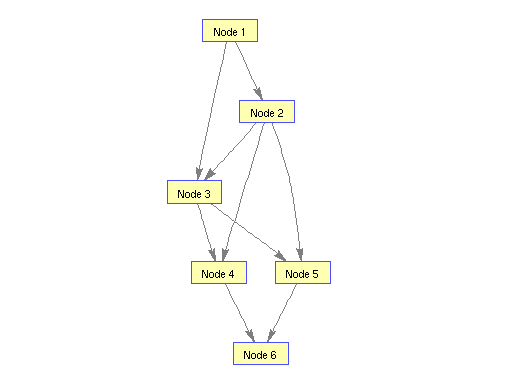
\includegraphics{images/testGraph}\caption{The test graph}
\end{figure}


I'm currently working on implementing this in MATLAB.
\begin{thebibliography}{1}
\bibitem{key-1} V. Reddy, 2015 - Sensor network design for contaminant
detection and identification in water distribution networks.

\bibitem{key-2}\href{http://link.springer.com/article/10.1007\%2FBF01581031}{On the structure of all min cuts in a network}

\bibitem{key-3}\href{http://dx.doi.org/10.1061/41203(425)32}{Optimization of Contaminant Sensor Placement in Water Distribution Networks: Multi-Objective Approach}

\bibitem{key-4}\href{http://files.waterky.org/aamastrrefs/Hart\%20and\%20Murray.\%202010.\%20Rev\%20of\%20\%20sensor\%20placem\%20strateg\%20for\%20contam\%20warn\%20systs\%20in\%20dr\%20wtr\%20dist\%20systs.\%20JWRPM\%20136.\%20611..pdf}{Review of Sensor Placement Strategies for Contamination Warning Systems in Drinking Water Distribution Systems}
10.1061/ ASCE WR.1943-5452.0000081

\bibitem{key-5}\href{http://doi:10.1016/j.proeng.2014.11.175}{Sensor Placement Methods for Contamination Detection in Water Distribution Networks: A Review}\end{thebibliography}

\end{document}
